\documentclass[tikz,border=4pt]{standalone}

\usepackage{amsmath,bm}
\usetikzlibrary{positioning,arrows.meta}

\tikzset{
  font=\sffamily,
  split/.style={draw, rounded corners, inner sep=.45em, fill=blue!15},
  leaf/.style={draw, rounded corners, inner sep=.45em, fill=green!15},
  edgelbl/.style={font=\sffamily\scriptsize, inner sep=1.5pt},
}

\begin{document}
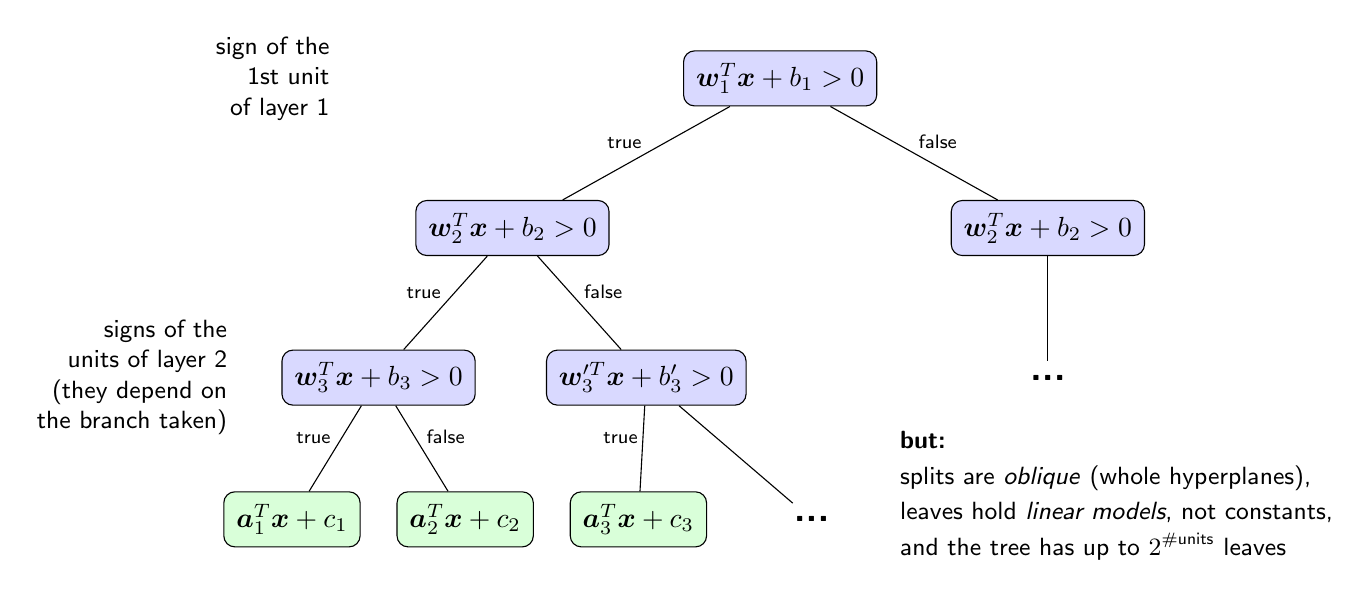
\begin{tikzpicture}[x=1cm, y=1cm]
  \node[split] (t1) at (0, 0)       {$\bm w_1^T \bm x + b_1 > 0$};
  \node[split] (t2) at (-3.4, -1.9) {$\bm w_2^T \bm x + b_2 > 0$};
  \node[split] (t3) at (3.4, -1.9)  {$\bm w_2^T \bm x + b_2 > 0$};
  \node[split] (t4) at (-5.1, -3.8) {$\bm w_3^T \bm x + b_3 > 0$};
  \node[split] (t5) at (-1.7, -3.8) {$\bm w_3'^T \bm x + b_3' > 0$};
  \node[font=\sffamily, scale=1.4] (d1) at (3.4, -3.8) {\textbf{...}};
  \node[leaf] (l1) at (-6.2, -5.6) {$\bm a_1^T \bm x + c_1$};
  \node[leaf] (l2) at (-4.0, -5.6) {$\bm a_2^T \bm x + c_2$};
  \node[leaf] (l3) at (-1.8, -5.6) {$\bm a_3^T \bm x + c_3$};
  \node[font=\sffamily, scale=1.4] (d2) at (0.4, -5.6) {\textbf{...}};

  \draw (t1) -- node[edgelbl, above left] {true} (t2);
  \draw (t1) -- node[edgelbl, above right] {false} (t3);
  \draw (t2) -- node[edgelbl, above left] {true} (t4);
  \draw (t2) -- node[edgelbl, above right] {false} (t5);
  \draw (t3) -- (d1);
  \draw (t4) -- node[edgelbl, above left] {true} (l1);
  \draw (t4) -- node[edgelbl, above right] {false} (l2);
  \draw (t5) -- node[edgelbl, above left] {true} (l3);
  \draw (t5) -- (d2);

  \node[font=\sffamily\small, anchor=west, align=left] at (1.4, -5.3)
    {\textbf{but:}\\[.2em]
     splits are \emph{oblique} (whole hyperplanes),\\[.2em]
     leaves hold \emph{linear models}, not constants,\\[.2em]
     and the tree has up to $2^{\#\text{units}}$ leaves};

  \node[font=\sffamily\small, anchor=east, align=right] at (-5.6, 0)
    {sign of the\\1st unit\\of layer 1};
  \node[font=\sffamily\small, anchor=east, align=right] at (-6.9, -3.8)
    {signs of the\\units of layer 2\\(they depend on\\the branch taken)};
\end{tikzpicture}
\end{document}
